\section{Mirror}


\begin{figure*}[t]
    \centering
    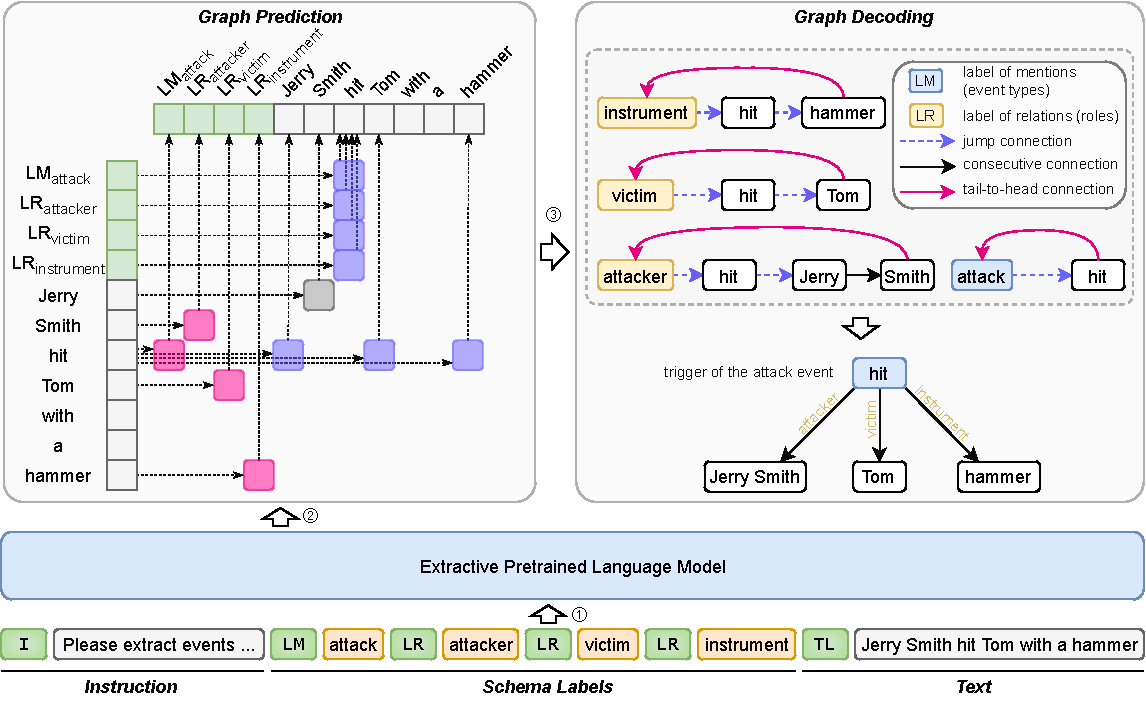
\includegraphics[width=\textwidth]{figs/Model Framework.pdf}
    \caption{Model framework (best viewed in color).}
    \label{fig:model-framework}
\end{figure*}

\subsection{Unified Data Interface}

To make the model able to handle different IE tasks, we propose a unified data interface for the input.
As shown in Figure~\ref{fig:model-framework}, there are three parts in the model input: the \textit{instruction}, the \textit{schema labels}, and the \textit{text}.
The instruction is composed of a leading token \verb|[I]| and a natural language sentence.
The leading token indicates the instruction part while the sentence tells the model what it should do.
For example, the instruction of NER could be \textit{Please identify any possible entities in the given text and label them with the following types}.
The instruction is the question in Machine Reading Comprehension (MRC) and Question Answering (QA) datasets.
For each task, we manually design a set of instructions, and randomly pick one of them for each training sample.
The number of instructions for each IE task is listed in Table~\ref{tab:pretrain-dataset-statistics}.

\begin{table}[t]
    \centering
    \begin{tabular}{lrrr}
        \toprule
        Task & \#Dataset & \#Instruction & \#Instance \\
        \midrule
        Cls &  & 42 &  \\
        MRC &  & 42 &  \\
        NER &  & 42 &  \\
        RE &  & 53 &  \\
        EE &  & 40 &  \\
        \bottomrule
    \end{tabular}
    \caption{Pretraining dataset statistics.}
    \label{tab:pretrain-dataset-statistics}
\end{table}

The schema labels are task ontologies that used for schema-guided extraction.
This part is consists of special token labels (\verb|[LM]|, \verb|[LR]| and \verb|LC|) and corresponding label texts.
Among the special tokens, \verb|[LM]| denotes the label of mentions (or event types), \verb|[LR]| denotes the label of relations (or argument roles), and \verb|[LC]| denotes the label of classes.
\verb|[LC]| token is designed for classification tasks when pretraining.

The text part is the input text that the model should extract information from.
It is composed of a leading token (\verb|[TL]| or \verb|[TP]|) and a natural language sentence.
If the leading token is \verb|[TL]|, the model should link labels from schema labels to spans in the text.
While the \verb|[TP]| token indicates the target spans are only in the text, and the model should extract information from the text without schema labels.
The \verb|[TP]| label is used in the pretraining stage to make the model able to extract information in MRC tasks without schema.
In classification tasks when pretraining, the model should not extract anything from the text part.
So we add a special background area with a leading token \verb|[B]| to distinguish from extractive texts.

With the above three parts, we can formulate classification, extractive MRC, multi-choice MRC, and IE tasks into a unified data interface, and the model can be trained in a unified way even the model is not based on generative language models.

\subsection{Multi-slot Tuple and Multi-span Cyclic Graph (MCG)}

We formulate IE tasks as a unified multi-span extraction problem.
For the flat NER task, the model is expected to extract a tuple like: ``((entity label position,), (span start position, span end position))''.
As shown in Figure~\ref{fig:multi-span-cyclic-graph} and the top right of Figure~\ref{fig:model-framework}, we formulate IE tasks into a unified multi-span cyclic graph, and regard labels as the leading tokens in schema labels.
There are three types of connections in the graph: the \textbf{\textit{consecutive}} connection, the \textbf{\color[HTML]{695efb} \textit{jump}} connection, and the \textbf{\color[HTML]{E9087F}\textit{tail-to-head}} connection.

The consecutive connection is used to \textbf{spans in the same entity}.
For an entity that has multiple tokens, the consecutive connection connects from the first token to the last token.
As shown in Figure~\ref{fig:model-framework}, ``Jerry'' connects to ``Smith''.
If there is only one token in an entity, the consecutive connection is not used.
For example, entities in ``muscle pain and fatigue'' contains two entities ``muscle pain'' and ``muscle fatigue''.
The consecutive connection is used to connect from ``muscle'' to ``pain'', and ``muscle'' to ``fatigue''.
The jump connection connects \textbf{different slots} in a tuple.
Schema labels and spans from texts are in different slots, so they are connected in jump connections.
In addition, the head entity and the tail entity of a relation triplet are in different slots, so they are also connected in jump connections.
The tail-to-head connection helps \textbf{locate the start \& end boundaries}, and forms a cycle in the graph.
It connects from the last token of the last slot to the first token of the first slot in a tuple.

\subsection{Model Structure}

With the unified data interface and the multi-span cyclic graph, we propose a unified model structure for IE tasks.
Similar to \citet{ner-as-dp}, we use biaffine attention to obtain the adjacency matrix of the multi-span cyclic graph.
For token representations $\mathbf{H}$, we get the adjacency matrix by Equation~\ref{eqn:biaffine}.


\begin{equation}
    \label{eqn:biaffine}
    \mathcal{\mathop{\odot}\limits_{i=1}^{n}} \mathbf{H} \mathbf{W}_{\text{biaffine}} \mathbf{H}^{\top} + \mathbf{H} \mathbf{W}_{\text{linear}} + \mathbf{W}_{\text{linear}}^{\top} \mathbf{H}^{\top} + \mathbf{W}_{\text{bias}}
\end{equation}
